\PassOptionsToPackage{unicode=true}{hyperref} % options for packages loaded elsewhere
\PassOptionsToPackage{hyphens}{url}
\documentclass[11pt,dvipsnames,ignorenonframetext,aspectratio=169]{beamer}
\IfFileExists{pgfpages.sty}{\usepackage{pgfpages}}{}
\setbeamertemplate{caption}[numbered]
\setbeamertemplate{caption label separator}{: }
\setbeamercolor{caption name}{fg=normal text.fg}
\beamertemplatenavigationsymbolsempty
\usepackage{lmodern}
\usepackage{amssymb,amsmath}
\usepackage{ifxetex,ifluatex}
\usepackage{fixltx2e} % provides \textsubscript
\ifnum 0\ifxetex 1\fi\ifluatex 1\fi=0 % if pdftex
  \usepackage[T1]{fontenc}
  \usepackage[utf8]{inputenc}
\else % if luatex or xelatex
  \ifxetex
    \usepackage{mathspec}
  \else
    \usepackage{fontspec}
\fi
\defaultfontfeatures{Ligatures=TeX,Scale=MatchLowercase}







\fi

  \usetheme[]{monash}

  \usecolortheme{monashwhite}


% A default size of 24 is set in beamerthememonash.sty

% Title page
\setbeamertemplate{title page}
{\placefig{-0.01}{-0.01}{width=1.01\paperwidth,height=1.01\paperheight}{carlzimmerobesity.png}
% \begin{textblock}{7.5}(1,2.8)\usebeamerfont{title} % original
\begin{textblock}{15}(1,2.2)\usebeamerfont{title}
{\color{white}\raggedright\par\inserttitle}
\end{textblock}
\begin{textblock}{10}(1,6)
\small
{\color{white}\raggedright{\insertauthor}\mbox{}\\[0.1cm]
\insertdate}
\end{textblock}}


  \useinnertheme{rounded}

  \useoutertheme{smoothtree}

% use upquote if available, for straight quotes in verbatim environments
\IfFileExists{upquote.sty}{\usepackage{upquote}}{}
% use microtype if available
\IfFileExists{microtype.sty}{%
  \usepackage{microtype}
  \UseMicrotypeSet[protrusion]{basicmath} % disable protrusion for tt fonts
}{}


\newif\ifbibliography


\hypersetup{
      pdftitle={Population genetics},
            colorlinks=true,
    linkcolor=red,
    citecolor=Blue,
    urlcolor=lightgrayd,
    breaklinks=true}
%\urlstyle{same}  % Use monospace font for urls







% Prevent slide breaks in the middle of a paragraph:
\widowpenalties 1 10000
\raggedbottom

  \AtBeginPart{
    \let\insertpartnumber\relax
    \let\partname\relax
    \frame{\partpage}
  }
  \AtBeginSection{
    \ifbibliography
    \else
      \let\insertsectionnumber\relax
      \let\sectionname\relax
      \frame{\sectionpage}
    \fi
  }
  \AtBeginSubsection{
    \let\insertsubsectionnumber\relax
    \let\subsectionname\relax
    \frame{\subsectionpage}
  }



\setlength{\parindent}{0pt}
\setlength{\parskip}{6pt plus 2pt minus 1pt}
\setlength{\emergencystretch}{3em}  % prevent overfull lines
\providecommand{\tightlist}{%
  \setlength{\itemsep}{0pt}\setlength{\parskip}{0pt}}

  \setcounter{secnumdepth}{0}


%% Monash overrides
\AtBeginSection[]{
   \frame<beamer>{
   \frametitle{Outline}\vspace*{0.2cm}
   
   \tableofcontents[currentsection,hideallsubsections]
  }}

% Redefine shaded environment if it exists (to ensure text is black)
\ifcsname Shaded\endcsname
  \definecolor{shadecolor}{RGB}{225,225,225}
  \renewenvironment{Shaded}{\color{black}\begin{snugshade}\color{black}}{\end{snugshade}}
\fi
%%

  \usepackage{setspace}
  \usepackage{wasysym}
  % \usepackage{footnote} % don't use this this breaks all
  \usepackage{fontenc}
  \usepackage{fontawesome}
  \usepackage{booktabs,siunitx}
  \usepackage{longtable}
  \usepackage{array}
  \usepackage{multirow}
  \usepackage{wrapfig}
  \usepackage{float}
  \usepackage{colortbl}
  \usepackage{pdflscape}
  \usepackage{tabu}
  \usepackage{threeparttable}
  \usepackage{threeparttablex}
  \usepackage[normalem]{ulem}
  \usepackage{makecell}
  \usepackage{xcolor}
  \usepackage{tikz} % required for image opacity change
  \usepackage[absolute,overlay]{textpos} % for text formatting
  \usepackage{chemfig}
  \usepackage[skip=0.333\baselineskip]{caption}
  % \newcommand*{\AlignChar}[1]{\makebox[1ex][c]{\ensuremath{\scriptstyle#1}}}%

  % this font option is amenable for beamer
  \setbeamerfont{caption}{size=\tiny}
  \singlespacing
  \definecolor{lightgrayd}{gray}{0.95}
  \definecolor{skyblued}{rgb}{0.65, 0.6, 0.94}
  \definecolor{oranged}{RGB}{245, 145, 200}

  \newlength{\cslhangindent}
  \setlength{\cslhangindent}{1.5em}
  \newenvironment{cslreferences}%
    {\setlength{\parindent}{0pt}%
    \everypar{\setlength{\hangindent}{\cslhangindent}}\ignorespaces}%
    {\par}

  \title[]{Population genetics}


  \author[
        Deependra Dhakal\\
College of Natural Resource Management\\
Agriculture and Forestry University\\
\textit{ddhakal.rookie@gmail.com}\\
\url{https://rookie.rbind.io}
    ]{Deependra Dhakal\\
College of Natural Resource Management\\
Agriculture and Forestry University\\
\textit{ddhakal.rookie@gmail.com}\\
\url{https://rookie.rbind.io}}


\date[
      
  ]{
    }

\begin{document}

% Hide progress bar and footline on titlepage
  \begin{frame}[plain]
  \titlepage
  \end{frame}


   \frame<beamer>{
   \frametitle{Outline}\vspace*{0.2cm}
   
   \tableofcontents[hideallsubsections]
  }

\hypertarget{evolution-and-evidences}{%
\section{Evolution and evidences}\label{evolution-and-evidences}}

\begin{frame}{Introduction to key terms}
\protect\hypertarget{introduction-to-key-terms}{}
\footnotesize

Mutations alter an organism's genotype and occasionally this causes
different phenotypes to appear. Most mutations have little effect on an
organism's phenotype, health, or reproductive fitness. Mutations that do
have an effect are usually detrimental, but occasionally some can be
beneficial. Studies in the fly \emph{Drosophila melanogaster} suggest
that if a mutation changes a protein produced by a gene, about 70
percent of these mutations will be harmful with the remainder being
either neutral or weakly beneficial.

\begin{itemize}
\tightlist
\item
  A population can be defined as a group of interbreeding individuals
  and their offspring.
\item
  Population genetics studies the distribution of genetic differences
  within populations and how these distributions change over time.
\item
  Changes in the frequency of an allele in a population are mainly
  influenced by \textbf{natural selection}.
\item
  Over many generations, the genomes of organisms can change
  significantly, resulting in evolution. In the process called
  \textbf{adaptation}, selection for beneficial mutations can cause a
  species to evolve into forms better able to survive in their
  environment.
\item
  New species are formed through the process of \textbf{speciation},
  often caused by geographical separations that prevent populations from
  exchanging genes with each other.
\item
  By comparing the homology between different species' genomes, it is
  possible to calculate the evolutionary distance (presented as
  evolutionary trees!) between them and when they may have diverged.
\item
  Genetic comparisons are more accurate than phenotypic.
\end{itemize}
\end{frame}

\begin{frame}{Theories of evolution}
\protect\hypertarget{theories-of-evolution}{}
\begin{columns}[T,onlytextwidth]
\column{0.4\textwidth}

The theory of \textbf{special creation} and the theory of \textbf{descent with modification} make different assertions about species, where they came from, and how they are related, as well as different assertions about the age of Earth. These assertions can be checked against evidence.

\column{0.6\textwidth}

\begin{figure}
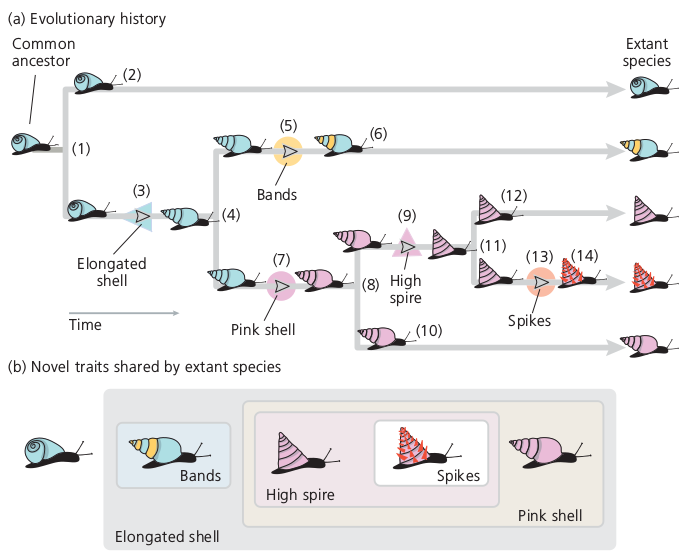
\includegraphics[width=0.78\linewidth]{../images/descent_with_modification_produces_nested_traits} \caption{\textbf{Testing theory of descent with modification with structural homology}. Descent with modification produces nested set of traits (a) The evolutionary history of a suite of hypothetical snail species. (b) The novel traits shared by the extant species.}\label{fig:descent-with-modification}
\end{figure}

\end{columns}
\end{frame}

\begin{frame}{}
\protect\hypertarget{section}{}
\begin{figure}
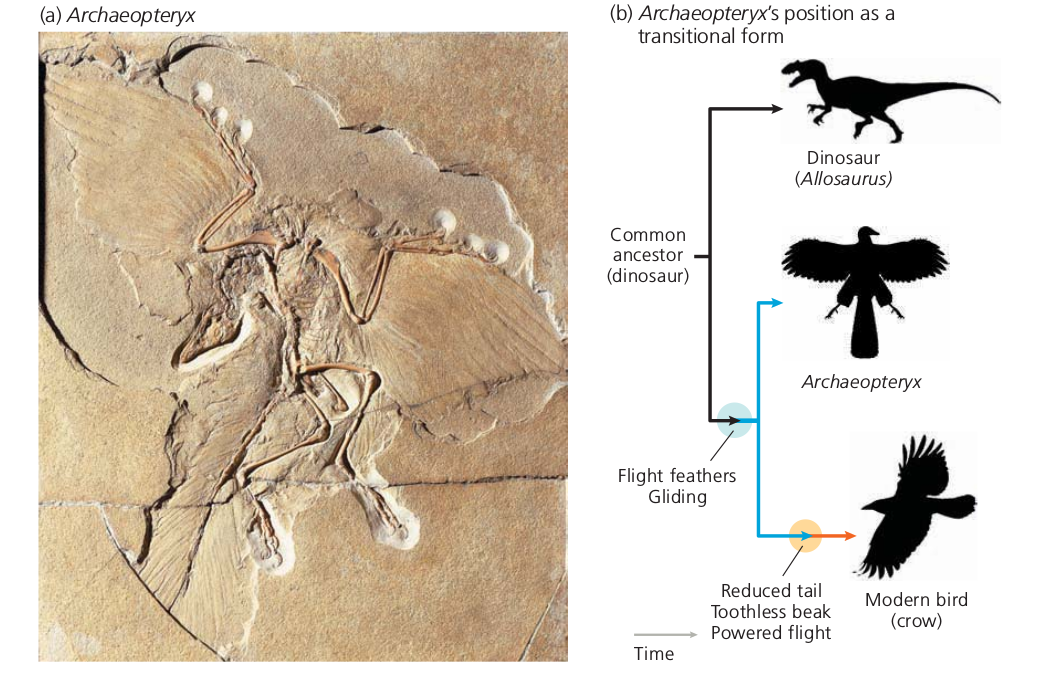
\includegraphics[width=0.6\linewidth]{./../images/modern_ancient_birds} \caption{A bird with a dinosaur's skeleton (a) Archaeopteryx had flight feathers like a modern bird's and a dinasaur-like skeleton with teeth and a long tail. (b) The distribution of traits in dinosaurs, birds, and Archaeopteryx is consistent with idea that they share an ancestor (Phylogeny simplified from Lloyd et al. 2008; Hu et al. 2009. Archaeopteryx reconstruction after Longrich 2006.))}\label{fig:tree-of-life}
\end{figure}
\end{frame}

\begin{frame}{Evidences for evolution}
\protect\hypertarget{evidences-for-evolution}{}
\begin{columns}[T,onlytextwidth]

\column{0.4\textwidth}

\begin{itemize}
\item Direct observation
\item Morphological homology
\item Developmental homology
\end{itemize}

\column{0.6\textwidth}


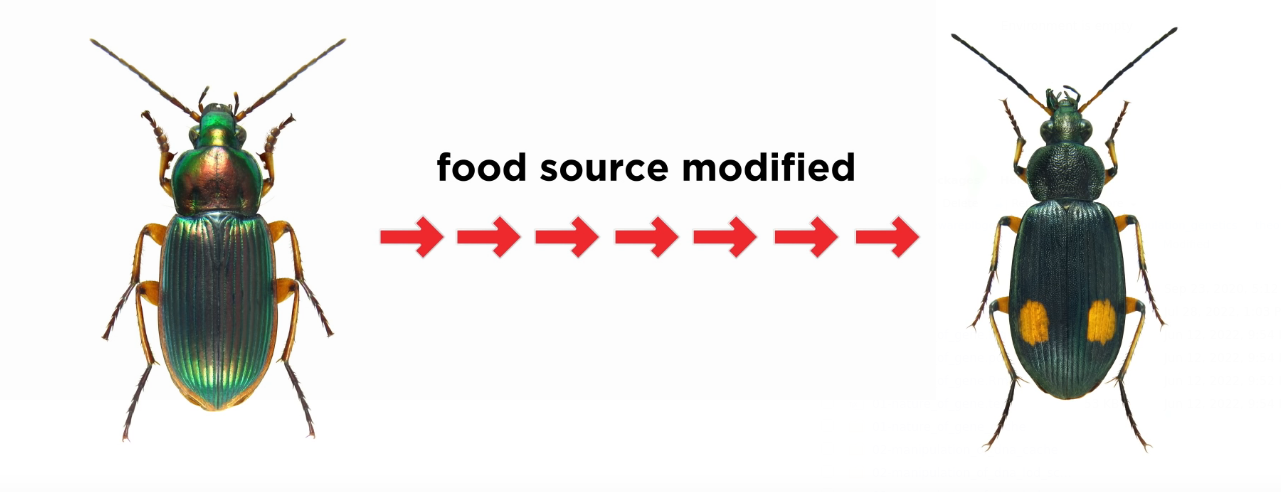
\includegraphics[width=0.9\linewidth]{../images/insect_fooding_changes_evolution} 


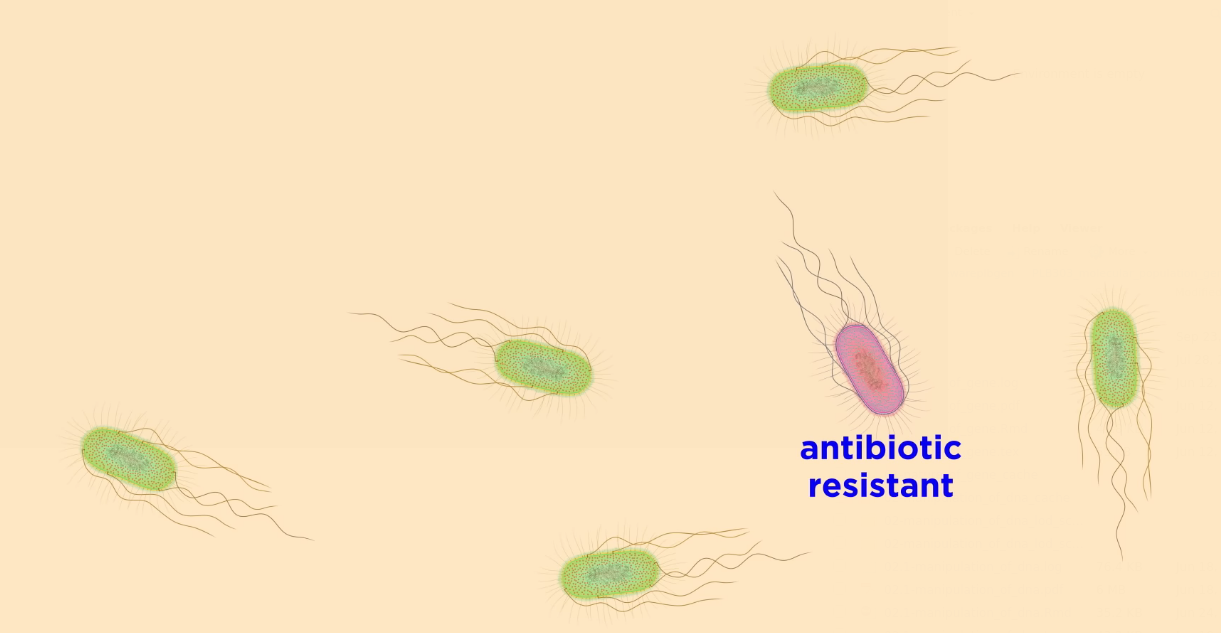
\includegraphics[width=0.85\linewidth]{../images/bacterial_antibiotic_resistance} 

\end{columns}
\end{frame}

\begin{frame}{}
\protect\hypertarget{section-1}{}
\begin{figure}
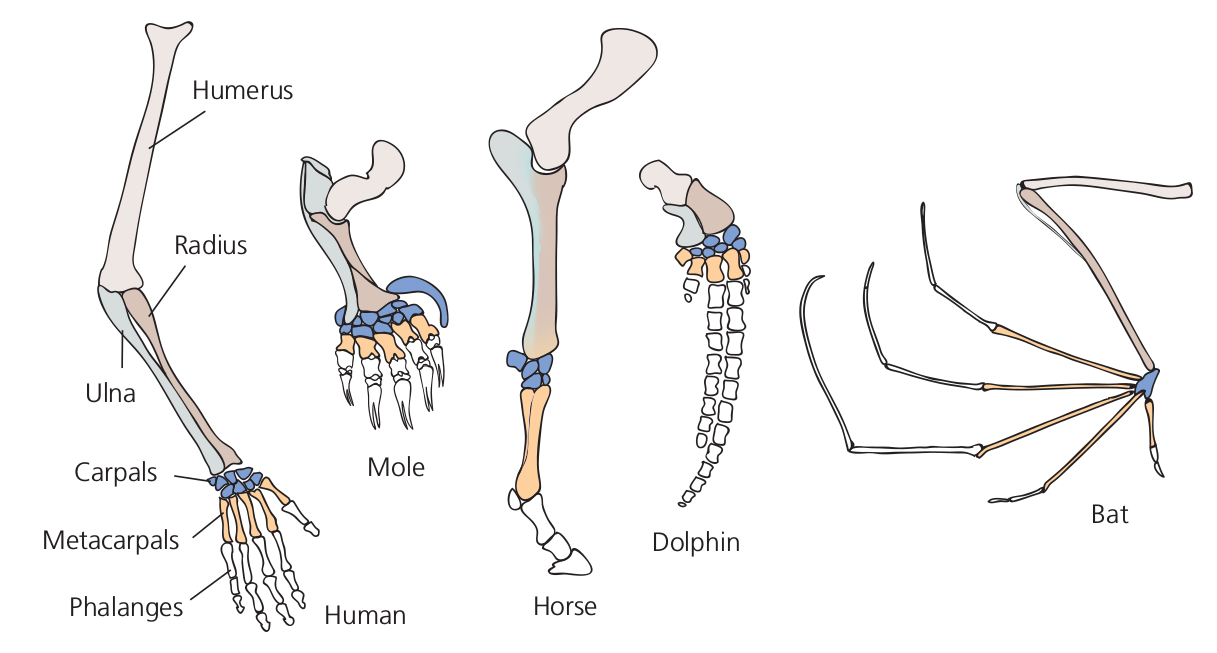
\includegraphics[width=0.86\linewidth]{../images/structural_homologies_bones_human_other} \caption{Structural homologies. These vertebrate forelimbs are used for different functions, but have the same sequence and arrangement of bones (Homologous bones are colored in the same way and are labelled on the human arm.)}\label{fig:structural-homologies-bones}
\end{figure}
\end{frame}

\begin{frame}{}
\protect\hypertarget{section-2}{}
\begin{columns}
\column{0.5\textwidth}
\begin{itemize}
\footnotesize
\item Carpels, stamens, petals, and sepals, are homologous with and derived from leaves. The development of these parts through a pattern of gene expression in the growing zones (meristems) is described by the ABC model of flower development. Each of the four types of flower parts is serially repeated in concentric whorls, controlled by a small number of genes acting in various combinations. Thus, A genes working alone result in sepal formation; A and B together produce petals; B and C together create stamens; C alone produces carpels. When none of the genes are active, leaves are formed. Two more groups of genes, D to form ovules and E for the floral whorls, complete the model. The genes are evidently ancient, as old as the flowering plants themselves.
\end{itemize}
\column{0.5\textwidth}


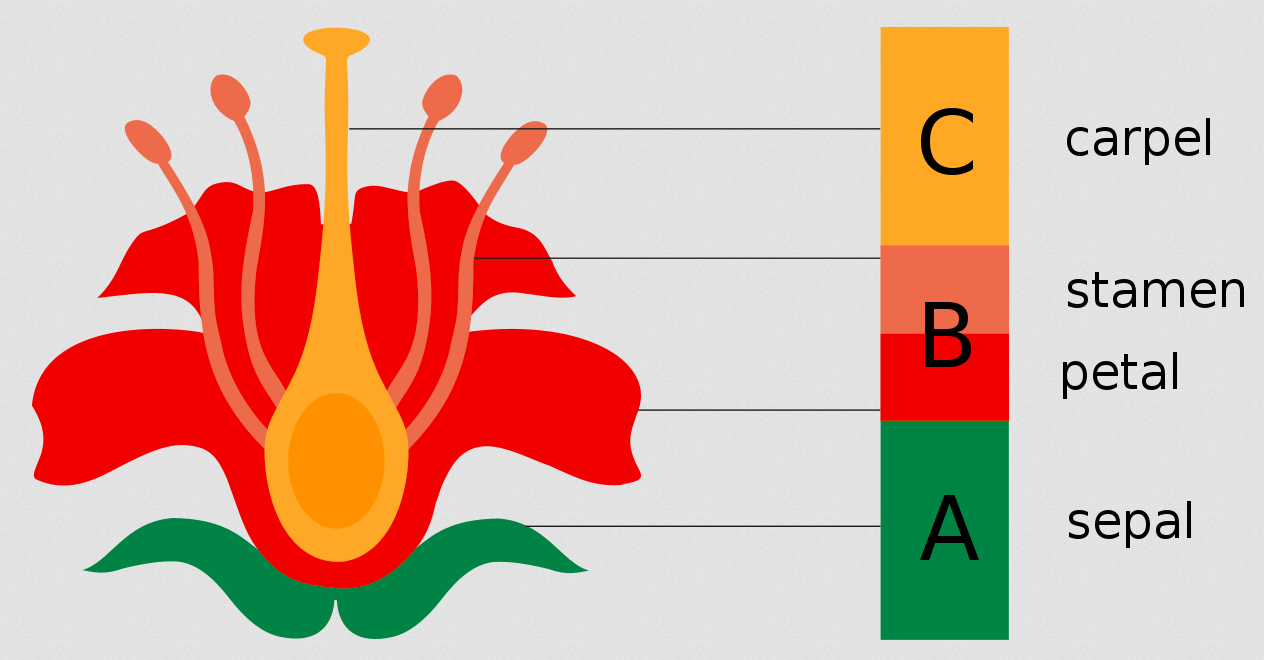
\includegraphics[width=0.98\linewidth]{../images/floral-parts-as-leaf-homologues} 

\end{columns}
\end{frame}

\begin{frame}{}
\protect\hypertarget{section-3}{}
\begin{columns}

\column{0.62\textwidth}
\textbf{\Large Sequence homology}
\begin{itemize}
\footnotesize
\item Vertebrates are the least diverse group; however, most vertebrates still possess a lot of nucleotide diversity. For humans, nucleotide diversity is about 0.001, meaning that two randomly chosen human chromosomes will differ at about 1 bp per thousand. With 3 billion bp in our genome, that adds up to a total of about 3 million differences between the set of chromosomes inherited from a person's mother and the set inherited from a person's father for non-inbred individuals.
\end{itemize}


\begin{center}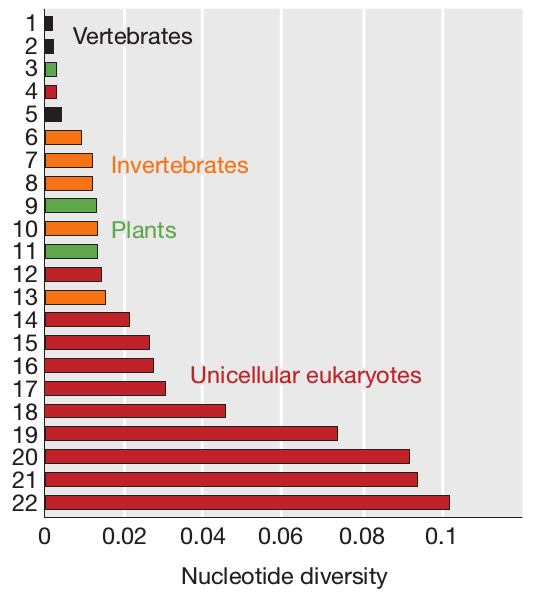
\includegraphics[width=0.36\linewidth]{../images/nucleotide_diversity_organisms} \end{center}

\column{0.38\textwidth}

\begin{figure}
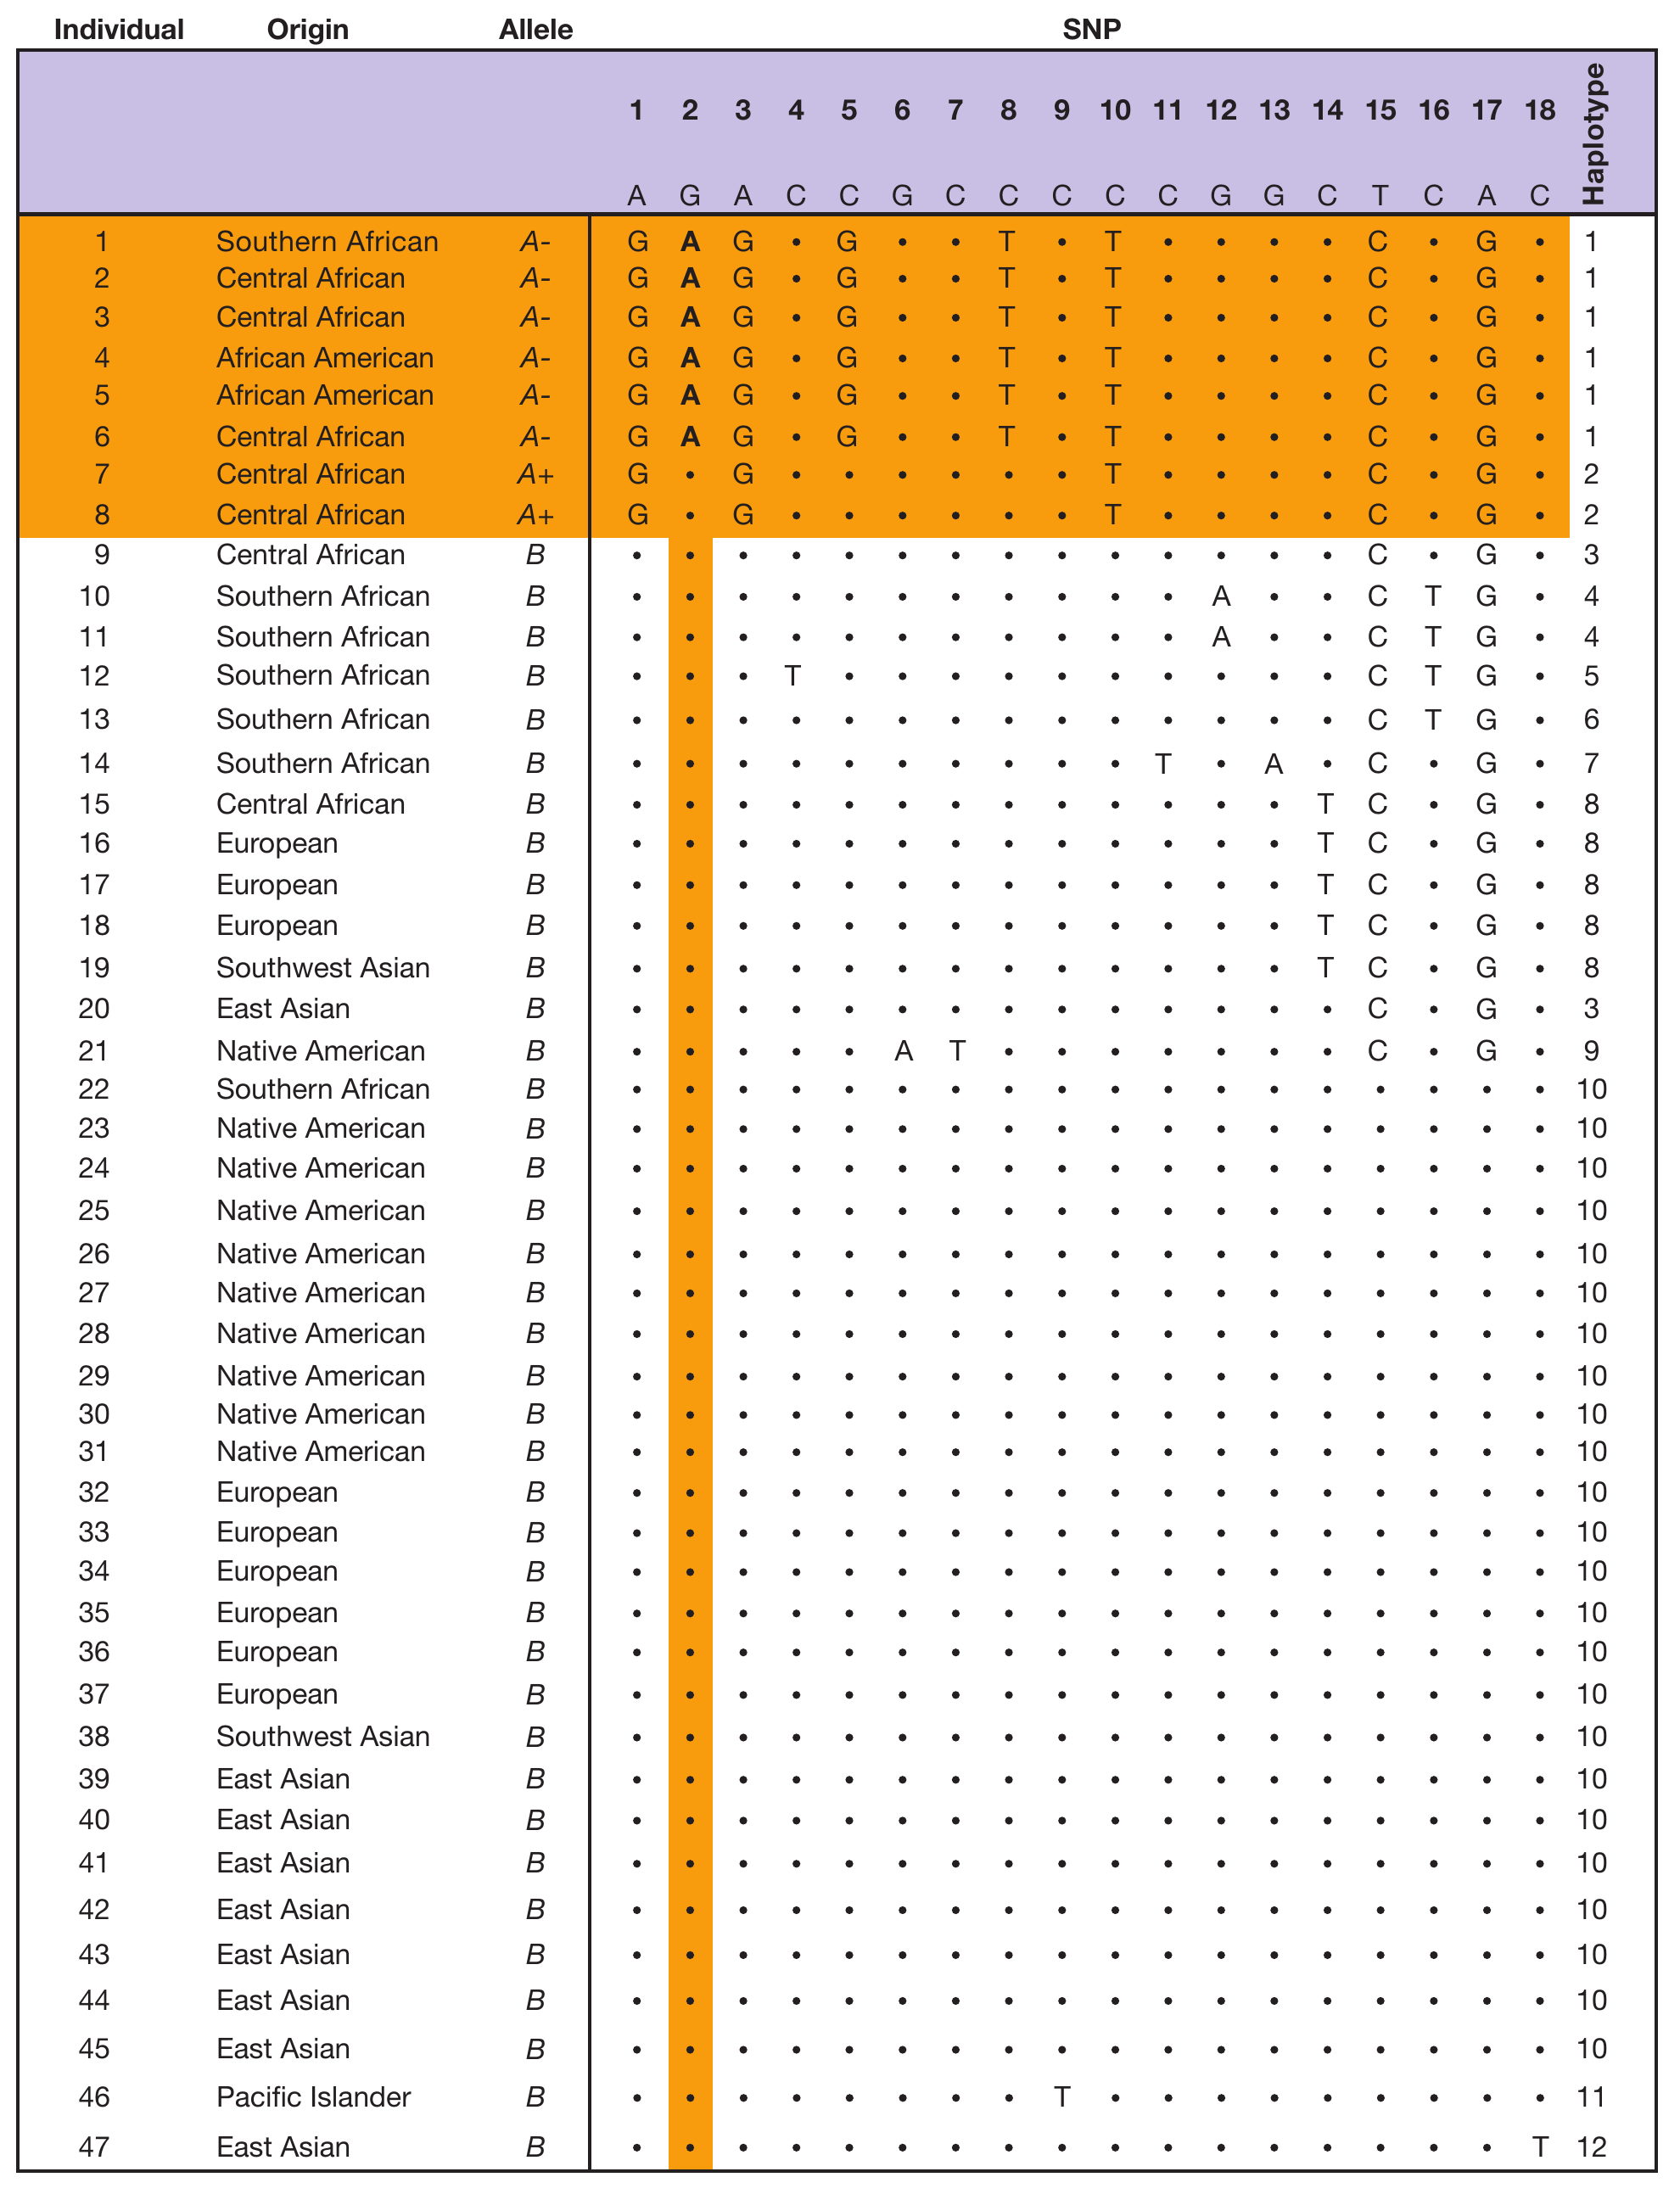
\includegraphics[width=0.99\linewidth]{../images/sequence_homology_variation_g6pd} \caption{Nucleotide variation for 5102 bp of the G6PD gene for a worldwide sample of 47 men. Only the 18 variable sites are shown. The functional allele classes (A-, A+, or B) is shown for each sequence. SNP2 is a non-sysnomymous SNP that causes a valine-to-methionine change that underlies differences in enzyme activity associated with the A- allele. SNP3 is a nonsynomymous SNP that causes an aspartic-acid-to-asparagine amino acid change. (Data from M.A. Saunders et al., Genetics 162, 2002, 1849-1861)}\label{fig:sequence-homology-g6pd-locus}
\end{figure}

\end{columns}
\end{frame}

\begin{frame}{}
\protect\hypertarget{section-4}{}
\begin{columns}

\column{0.35\textwidth}

\begin{itemize}
\item Vestigeal organs
\item Fossil records
\end{itemize}

\column{0.65\textwidth}


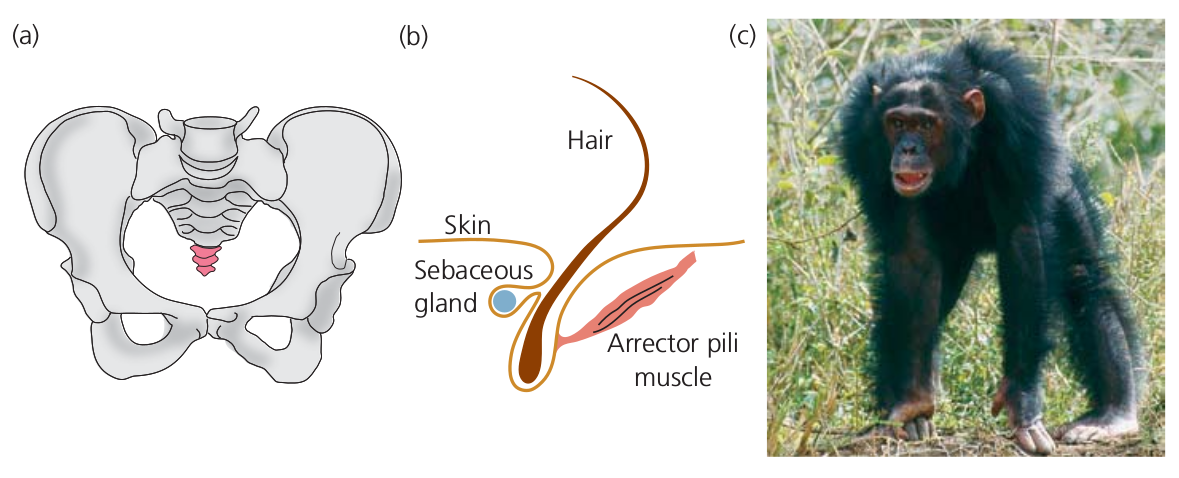
\includegraphics[width=0.95\linewidth]{../images/vestigeal_traits_coccyx_arrector_pili} 

\end{columns}
\end{frame}

\hypertarget{populations-structure-stratification-and-evolution-by-natural-selection}{%
\section{Populations structure, stratification and evolution by natural
selection}\label{populations-structure-stratification-and-evolution-by-natural-selection}}

\begin{frame}{Natural population}
\protect\hypertarget{natural-population}{}
\begin{itemize}
\tightlist
\item
  Natural population are subject to variable conditions of mutation,
  migration, and selection. They are non constant with respect to size,
  mating pattern.
\item
  Multiple loci and multiple alleles per loci interact to cause variable
  fitness of genotypes.
\item
  Most popular approach to studying natural population is to make
  measurements of various characteristics present in natural and
  experimental (hypothesized) population and then, in combination with
  mathematical analysis, use these observations to derive the genetic
  structure of populations.
\end{itemize}
\end{frame}

\begin{frame}{Optimum phenotypes and selection pressure}
\protect\hypertarget{optimum-phenotypes-and-selection-pressure}{}
\begin{itemize}
\tightlist
\item
  Because of selection over long period of time, most populations may be
  considered to have achieved phenotypes optimally adapted to their
  surroundings.
\item
  Large number of phenotypes cluster around value of highest fitness.
\item
  ``It is quite as dangerous to be conspicuously above a certain
  standard of organic excellence as it is to be conspicuously below the
  standard'' (Bumpus, 1899; The elimination of the unfit as illustrated
  by the introduced sparrows.)
\end{itemize}

\begin{table}

\caption{\label{tab:optimal-birth-weight-human}\textbf{Optimal birth weight in human}. Proportion of suvivors (1 month after) of the female birth at London hospital. Optimal birth weight, that which has highest proportion of survivors is 8 pounds.}
\centering
\fontsize{8}{10}\selectfont
\begin{tabular}[t]{rrr}
\toprule
Total Female Births & Survivors After 1Mo & Dead At 1Mo\\
\midrule
6693 & 6419 & 274\\
\bottomrule
\end{tabular}
\end{table}
\end{frame}

\begin{frame}{}
\protect\hypertarget{section-5}{}
\footnotesize

\begin{itemize}
\tightlist
\item
  In the present case, \(\longrightarrow\) Overall mortality = 4\%
  (mortality of optimum 8-pound class was only 1.2 \%). In other words,
  \(4.1 - 1.2 = 2.9\) percent additional mortality occurred in the
  population among the phenotypes which were not of the optimal 8-pound
  class. This 2.9 percent value may therefore be used as a measure of
  the intensity or pressure of selection for an optimum birth weight.
\item
  \textbf{Selection intensity} (I) can be defined as the difference in
  survival rates between optimal (\(S_0\)) and suboptimal (\(S_s\))
  phenotypes, multiplied by the frequency of suboptimal phenotypes
  (\(f_s\)).
\end{itemize}

\[
I = (S_o - S_s)\times f_s
\]

\begin{itemize}
\tightlist
\item
  When selection pressure is 0, all phenotypes are optimal
  (\(f_s = 0\)), and when selection pressure is 1, all phenotypes are
  sub-optimal with a survival rate zero (\(S_o - S_s = 1\)).
\item
  In London hospital birth case, \(S_o = \frac{718}{727} = .988\),
  \(S_s = \frac{5701}{5966} = .956\) and
  \(f_s = \frac{5966}{727+5966} = 0.892\), hence
\end{itemize}

\[
I = (0.988 - 0.956)\times 0.892 = 0.029
\]

\begin{itemize}
\tightlist
\item
  There was a total of 4.1\% deaths, of which 2.9\% were caused by
  selection against suboptimal phenotypes, or \(\frac{2.9}{4.1} = 70.8\)
  percent deaths were caused by selection against these phenotypes at
  birth.
\end{itemize}
\end{frame}

\begin{frame}{}
\protect\hypertarget{section-6}{}
\begin{figure}
\includegraphics[width=0.7\linewidth]{07-population_genetics_files/figure-beamer/natural-selection-for-optimal-phenotypes-1} \caption{Selection pressure on a population (I) under different frequencies of suboptimal phenotypes ($f_s$) and different departures of the suboptimal survival rate from the optimal ($S_o - S_s$)}\label{fig:natural-selection-for-optimal-phenotypes}
\end{figure}
\end{frame}

\begin{frame}{}
\protect\hypertarget{section-7}{}
\begin{itemize}
\tightlist
\item
  Value of \(S_o - S_s\) and \(f_s\) vary between different populations
  and undoubtedly at different times in the life cycle of any
  population.
\item
  High selection intensities do not persist for many generations , since
  any increase in \(I\) because of a new departure from optimum
  phenotype is an additional burden on a population that is already
  suffering from mortality caused by the usual non-selective factors
  that affect all phenotypes equally.
\end{itemize}
\end{frame}

\begin{frame}{Population size and inbreeding}
\protect\hypertarget{population-size-and-inbreeding}{}
\footnotesize

\begin{itemize}
\tightlist
\item
  In small populations, individuals are more likely to mate with a
  relative than in large ones. So, effect of population size on the
  overall level of inbreeding (as measured by
  \(F\)\footnote[frame]{"Inbreeding Coefficient" for pedigrees was derived in Chapter "Quantative Genetics".})
\item
  Consider a population with \(F_t\) being the level of inbreeding at
  generation \(t\). To form an individual in the next generation
  \(t + 1\), we select the first allele from the gene pool. Suppose the
  population size is \(N\).
\item
  After the first allele is selected, the probability that the second
  allele we pick will be exactly the same copy is 1/2N and the
  inbreeding coefficient for this individual is 1.
\item
  The probability that the second allele we pick will be different copy
  from the first allele is \(1 - \frac{1}{2}N\) and the level of
  inbreeding for the resulting individual would be \(F_t\), the average
  inbreeding coefficient for the initial population at generation \(t\).
\item
  The level of inbreeding in the next generation is the sum of these two
  possible outcomes:
\end{itemize}

\[
\small
F_{t+1} = \frac{1}{2N}1 + \left(1 - \frac{1}{2N}\right)F_t
\]
\end{frame}

\begin{frame}{}
\protect\hypertarget{section-8}{}
\footnotesize

\begin{itemize}
\tightlist
\item
  This shows that \(F\) will increase over time as function of
  population size.

  \begin{itemize}
  \tightlist
  \item
    When \(N\) is large, \(F\) increases slowly over time.
  \item
    When \(N\) is small, \(F\) increases rapidly over time.
  \end{itemize}
\item
  The equation above can be re-written as:
\end{itemize}

\[
\small
(1 - F_{t+1}) = \left(1 - \frac{1}{2N} \right) (1 - F_t)
\]
\end{frame}

\begin{frame}{}
\protect\hypertarget{section-9}{}
\begin{itemize}
\tightlist
\item
  We also have the formula for the frequency of heterozygotes (\(H\))
  with inbreeding as,
\end{itemize}

\[
\small
\begin{aligned}
& H = f_{A/a} &=& 2pq - 2pqF \\
\implies & (1-F) &=& \frac{H}{2pq}
\end{aligned}
\]

\begin{itemize}
\tightlist
\item
  Combining these two equations, we get:
\end{itemize}

\[
\small
\begin{aligned}
& \frac{H_{t+1}}{2pq}  &=& \left( 1- \frac{1}{2N} \right) \frac{H_t}{2pq}\\
\implies &(H_{t+1}) &=& \left(1 - \frac{1}{2N} \right) H_t
\end{aligned}
\]
\end{frame}

\begin{frame}{}
\protect\hypertarget{section-10}{}
\footnotesize

\begin{itemize}
\tightlist
\item
  Thus, for each generation, the level of heterozygosity is reduced by
  the fraction (\(1 - \frac{1}{2N}\)). The reduction in H over \(t\)
  generations can be combined with the change in \(F\) over generations
  as,
\end{itemize}

\[
F_t = 1 - \left(1 - \frac{1}{2N} \right)^t (1 - F_0)
\]

\begin{center}\includegraphics[width=0.6\linewidth]{07-population_genetics_files/figure-beamer/increasing-inbreeding-over-time-for-N-1} \end{center}
\end{frame}

\begin{frame}{Types of selection}
\protect\hypertarget{types-of-selection}{}
\begin{itemize}
\tightlist
\item
  Stabilizing selection
\item
  Directional selection (common in plant/animal breeding)
\item
  Cyclical selection
\item
  Disruptive selection
\end{itemize}

\begin{figure}
\includegraphics[width=0.7\linewidth]{07-population_genetics_files/figure-beamer/selection-types-1} \caption{Stabilizing and directional selection types. Parents in the shaded region are selected for producing the next generation.}\label{fig:selection-types}
\end{figure}
\end{frame}

\hypertarget{gene-and-genotypes}{%
\section{Gene and genotypes}\label{gene-and-genotypes}}

\begin{frame}{Mendel's model of particulate genetics}
\protect\hypertarget{mendels-model-of-particulate-genetics}{}
\begin{itemize}
\tightlist
\item
  Mendel's first law (Aa): independent segregation of alleles at a
  single locus occurs due to random sampling without bias
\end{itemize}

\begin{itemize}
\tightlist
\item
  Mendel's second law (AaBb): independent assortment of multiple loci is
  due to various linkage groups (apply the product rule)
\end{itemize}
\end{frame}

\begin{frame}{What is allele/gene ?}
\protect\hypertarget{what-is-allelegene}{}
An allele/gene is the bit of DNA at the place called locus (the place on
a chromosome where an allele resides). An allele is instantiation of a
locus. But by orthology, a locus is not template for an allele.
Similarly, a locus is not tangible, rather a map describing where to
find a tangible thing, an allele on a chromosome. A diploid individual
has two alleles at a particular autosomal locus.
\end{frame}

\begin{frame}{Genotype and allele frequencies}
\protect\hypertarget{genotype-and-allele-frequencies}{}
In A loci, suppose, two alleles \(A_1\) and \(A_2\) are present in a
diploid organism the genotype and genotypic frequency of segregating
population will be;

\[
\begin{aligned}
\textrm{Genotype} \hspace{20pt} & A_1A_1 & A_1A_2 \hspace{20pt} & A_2A_2 \\
\textrm{Relative frequency} \hspace{20pt} & x_{11} & x_{12} \hspace{20pt} & x_{22}
\end{aligned}
\]

As, relative frequencies must add to 1,

\[
x_{11} + x_{12} + x_{22} = 1
\]

The order of subscripting heterozygous is arbitrary.

Frequency of \(A_1\) allele in the population is,

\[
p = x_{11} + \frac{1}{2}x_{12}
\]
\end{frame}

\begin{frame}{}
\protect\hypertarget{section-11}{}
and frequency of \(A_2\) allele is,

\[
q = 1-p = x_{22} + \frac{1}{2}x_{12}
\]

Measure of each allele frequency can be thought of as independent
events. For e.g., for allele \(p\) to be selected;

\[
p = \left(x_{11} \times \frac{1}{P(p_{A_1A_1})}\right) + \left(x_{12} \times \frac{1}{2}\right) + (x_{22} \times 0)
\]

Where, \(P(p, A_1A_1)\) is the probability of getting \(p\) allele from
\(A_1A_1\) genotype, for loci with more than two alleles, frequency of
\(i^{th}\) allele will be called \(p_i\). Frequency of \(A_iA_j\)
genotype will be called \(x_{ij}\) for heterozygotes, \(i\neq j\) and,
by convention, \(i<j\).
\end{frame}

\begin{frame}{}
\protect\hypertarget{section-12}{}
If there are \(n\) alleles,

\[
\begin{aligned}
1 &= x_{11} + x_{22} + x_{33} + ... + x_{nn} + x_{12} + x_{13} + x_{(n-1)n} \\
  &= \sum^n_{i=1}\sum^n_{j\geq i}{x_{ij}}
\end{aligned}
\]

The frequency of \(i^{th}\) allele is

\[
p_i = x_{ii} + \frac{1}{2}\sum^{i-1}_{j = 1}{x_{ji}} + \frac{1}{2}\sum^n_{j = i+1}{x_{ij}}
\]
\end{frame}

\begin{frame}{}
\protect\hypertarget{section-13}{}
\scriptsize

In a population consisting of 10,000 individuals, 1 individual is of
``aa'' genotype. If the population is in Hardy-Weinberg equilibrium,
find the gene and genotype frequencies of that population.

Total population (\(N\)) = 10000

Number of individuals of \(aa\) genotype = 1

Since the population is in HW equilibrium, gene and genotype frequencies
of the population stay constant over generations, i.e.

Gene frequencies = \(p^2 + q^2 = 1\), and

Genotype frequencies = \(p^2AA + 2pqAa + q^2aa = 1\)

So,

\(\rightarrow\) genotype frequency of homozygous recessive
\(aa\)(\(q^2\)) = \(\frac{1}{10000}\) = \ensuremath{10^{-4}}

\(\rightarrow\) gene frequency of minor allele \(a\)(\(q\)) =
\(\sqrt{\frac{1}{10000}}\) = 0.01

\(\rightarrow\) gene frequency of major allele \(A\)(\(p\)) = \(1 - p\)
= 0.99

\(\rightarrow\) genotype frequency of heterogygous \(Aa\)(\(2pq\)) =
0.02

\(\rightarrow\) genotype frequency of homozygous dominant
\(AA\)(\(p^2\)) = 0.98
\end{frame}

\hypertarget{hardy-weinberg-law}{%
\section{Hardy-Weinberg law}\label{hardy-weinberg-law}}

\begin{frame}{}
\protect\hypertarget{section-14}{}
\begin{itemize}
\tightlist
\item
  In a random mating population (in which each male gamete has an equal
  chance of mating with any female gamete), when taken a loci with
  differences in alleles (A/a), following genotypes are possible:
  \(AA\), \(Aa\) and \(aa\).
\item
  With the corresponding frequencies of \(p^2\), \(2pq\) and \(q^2\),
  respectively for each of the genotypes, and bearing that gene
  frequencies must add up to unity, \(p^2+2pq+q^2 = 1\). This
  mathematical relationship is called the \textbf{Hardy-Weinberg
  equilibrium}.
\item
  Two scientists showed that the frequency of genotypes in a population
  depends on the frequency of genes in the preceding generation, not on
  the frequency of the genotypes.
\item
  HW equation: \(p^2 + 2pq + q^2 =1\)
\item
  HW equilibrium: \(f(A)_t = f(A)_{t+1}\)
\item
  Genotype frequencies remain constant over generations as long as the
  assumptions of HW are met.
\end{itemize}
\end{frame}

\begin{frame}{Hardy-Weinberg expected genotype frequency}
\protect\hypertarget{hardy-weinberg-expected-genotype-frequency}{}
\begin{figure}[center]
\includegraphics[width=0.7\linewidth]{07-population_genetics_files/figure-beamer/hw-expectation-in-frequencies-1} \caption{Attainment of HW-equilibrium in a diploid population shown across different values of starting allele frequencies (An example scenario with starting allele frequencies f(A) = 0.2 and f(a) = 0.8 is shown as marked.)}\label{fig:hw-expectation-in-frequencies}
\end{figure}
\end{frame}

\begin{frame}{Applications of HW}
\protect\hypertarget{applications-of-hw}{}
\begin{itemize}
\tightlist
\item
  Assume HW to compare two genetic models
\item
  Apply HW to estimate the freq of an observed genotype in a forensic
  DNA typing case
\item
  The \(\chi^2\) test gauges whether observed and expected differ more
  than expected by chance if the null hypothesis is true.
\end{itemize}
\end{frame}

\begin{frame}{}
\protect\hypertarget{section-15}{}
\begin{itemize}
\tightlist
\item
  In each subsequent generation following thereafter, however, gene and
  genotypic frequencies will remain unchanged, provided that:

  \begin{enumerate}
  \tightlist
  \item
    Random mating occurs in a very large diploid population;
  \item
    Allele A and allele a are equally fit (one does not confer a
    superior trait than the other);
  \item
    There is no differential migration of one allele into or out of the
    population;
  \item
    The mutation rate of allele A is equal to that of allele a.
  \end{enumerate}
\end{itemize}
\end{frame}

\begin{frame}{Conservation of gene frequencies}
\protect\hypertarget{conservation-of-gene-frequencies}{}
\small

\begin{itemize}
\tightlist
\item
  Let us presume that among humans, the difference between those who can
  and those who cannot taste the chemical phenyl-thiocarbamate (PTC)
  resides in a single gene difference with two alleles, \(T\) and \(t\).
\item
  The allele for tasting, \(T\), is dominant over \(t\), so that
  heterozygotes, \(Tt\) are tasters, and the only nontasters are \(tt\).
\item
  If we were to choose an initial population composed of an arbitary
  number of each genotype, we may ask what will be the frequency of
  these genes after many generations.
\item
  Let us, for example, place upon an island a group of children in the
  ratio \(.40TT:.40Tt:.20tt\). The gene frequencies in this newly formed
  population are therefore, \(.4 + .2 = .6 T\), and \(.2 + .2 = .4t\).
\item
  Let us also assume that the number of individuals in the population is
  large, and the tasting or nontasting has no effect upon survival
  (viability), fertility, or attraction between the sexes.
\end{itemize}
\end{frame}

\begin{frame}{}
\protect\hypertarget{section-16}{}
\begin{itemize}
\tightlist
\item
  As these children mature, they will choose their mates at random from
  those of the opposite sex regardless of their tasting abilities.
\item
  Matings between any two genotypes can then be predicted solely on the
  basis of the frequency of those genotypes in the population.
\item
  Table \ref{tab:random-mating-monogene-gene-freq} shows matings in all
  possible combination.
\end{itemize}

\begin{table}

\caption{\label{tab:random-mating-monogene-gene-freq}Types of random-mating combinations and their relative frequencies in a population containing .40TT, .40Tt, and .20tt genotypes}
\centering
\fontsize{8}{10}\selectfont
\begin{tabular}[t]{lrrr}
\toprule
gametes & TT & Tt & tt\\
\midrule
TT & 0.16 & 0.16 & 0.08\\
Tt & 0.16 & 0.16 & 0.08\\
tt & 0.08 & 0.08 & 0.04\\
\bottomrule
\end{tabular}
\end{table}
\end{frame}

\begin{frame}{}
\protect\hypertarget{section-17}{}
\begin{table}

\caption{\label{tab:unnamed-chunk-1}Relative frequencies of the different kinds of offspring produced by the matings}
\centering
\begin{tabular}[t]{lrlll}
\toprule
\multicolumn{2}{c}{Parents} & \multicolumn{3}{c}{Offspring ratio} \\
\cmidrule(l{3pt}r{3pt}){1-2} \cmidrule(l{3pt}r{3pt}){3-5}
Type of mating & Frequency of mating & TT & Tt & tt\\
\midrule
\cellcolor{gray!6}{$TT \times TT$} & \cellcolor{gray!6}{0.16} & \cellcolor{gray!6}{all(.16)} & \cellcolor{gray!6}{} & \cellcolor{gray!6}{}\\
$TT \times Tt$ & 0.32 & 1/2(.32) & +1/2(.32) & \\
\cellcolor{gray!6}{$TT \times tt$} & \cellcolor{gray!6}{0.16} & \cellcolor{gray!6}{} & \cellcolor{gray!6}{all (.16)} & \cellcolor{gray!6}{}\\
$Tt \times Tt$ & 0.16 & 1/4(.16) & +1/2 (.16) & +1/4(.16)\\
\cellcolor{gray!6}{$Tt \times tt$} & \cellcolor{gray!6}{0.16} & \cellcolor{gray!6}{} & \cellcolor{gray!6}{1/2(.16)} & \cellcolor{gray!6}{+1/2(.16)}\\
\addlinespace
$tt \times tt$ & 0.04 &  &  & all (.04)\\
\bottomrule
\end{tabular}
\end{table}
\end{frame}

\begin{frame}{}
\protect\hypertarget{section-18}{}
\begin{itemize}
\tightlist
\item
  Note that although the frequencies of genotypes have been altered by
  random mating, the gene frequencies have not changed.
\item
  For the \(T\) gene frequency is equal to \(.36 + 1/2(.48) = .60\), and
  the frequency of \(t\) is \(.16 + 1/2(.48) = .40\).
\item
  No matter what the initial frequencies of the three genotypes, the
  gene frequencies of the next generation will be the same as those of
  parental generation.
\end{itemize}
\end{frame}

\begin{frame}{Assertion}
\protect\hypertarget{assertion}{}
\begin{enumerate}
\tightlist
\item
  Under conditions of random mating ( \emph{panmixis}) in a large
  population where all genotypes are equally viable, gene frequencies of
  a particular generation depend upon the gene frequencies of the
  previous generation and not upon the \emph{genotype frequencies}.
\item
  The frequencies of different genotypes produced through random mating
  depend only upon the gene frequencies.
\end{enumerate}

\begin{itemize}
\tightlist
\item
  After the first generation of random mating, genotype frequencies also
  remain stable. i.e., equilibrium.
\end{itemize}
\end{frame}

\begin{frame}{Formal proof}
\protect\hypertarget{formal-proof}{}
\begin{table}

\caption{\label{tab:unnamed-chunk-2}Mating combinations and frequencies of offspring produced under conditions of random mating when genotypic frequencies are $p^2TT$, $2pqTt$, and $q^2tt$}
\centering
\fontsize{6}{8}\selectfont
\begin{tabular}[t]{>{\raggedright\arraybackslash}p{6em}>{\raggedright\arraybackslash}p{12em}>{\raggedright\arraybackslash}p{8em}>{\raggedright\arraybackslash}p{8em}>{\raggedright\arraybackslash}p{8em}}
\toprule
\multicolumn{2}{c}{Parents} & \multicolumn{3}{c}{Offspring ratio} \\
\cmidrule(l{3pt}r{3pt}){1-2} \cmidrule(l{3pt}r{3pt}){3-5}
Type of mating & Frequency of mating & TT & Tt & tt\\
\midrule
\cellcolor{gray!6}{$TT \times TT$} & \cellcolor{gray!6}{$p^2 \times p^2 = p^4$} & \cellcolor{gray!6}{$p^4$} & \cellcolor{gray!6}{} & \cellcolor{gray!6}{}\\
$TT \times Tt$ & $2 \times p^2 \times 2pq = 4p^3q$ & $2p^3q$ & $2p^3q$ & \\
\cellcolor{gray!6}{$TT \times tt$} & \cellcolor{gray!6}{$2 \times p^2 \times q^2 = 2p^2q^2$} & \cellcolor{gray!6}{} & \cellcolor{gray!6}{$2p^2q^2$} & \cellcolor{gray!6}{}\\
$Tt \times Tt$ & $2pq \times 2pq = 4p^2q^2$ & $p^2q^2$ & $2p^2q^2$ & $p^2q^2$\\
\cellcolor{gray!6}{$Tt \times tt$} & \cellcolor{gray!6}{$2 \times 2pq \times q^2 = 4pq^3$} & \cellcolor{gray!6}{} & \cellcolor{gray!6}{$2pq^3$} & \cellcolor{gray!6}{$2pq^3$}\\
\addlinespace
$tt \times tt$ & $q^2 \times q^2 = q^4$ &  &  & $q^4$\\
\midrule
\cellcolor{gray!6}{} & \cellcolor{gray!6}{$p^2(p^2 + 2pq + q^2) + 2pq(p^2 + 2pq + q^2) + q^2(p^2 + 2pq + q^2) = p^2 + 2pq + q^2 = (p + q)^2 = 1$} & \cellcolor{gray!6}{$p^4 + 2p^3q + p^2q^2 = p^2(p^2 + 2pq + q^2) = p^2$} & \cellcolor{gray!6}{$2p^3q + 4p^2q^2 + 2pq^3 = 2pq(p^2 + 2pq + q^2) = 2pq$} & \cellcolor{gray!6}{$p^2q^2 + 2pq^3 + q^4 = q^2(p^2 + 2pq + q^2) = q^2$}\\
\bottomrule
\end{tabular}
\end{table}
\end{frame}

\begin{frame}{Problem}
\protect\hypertarget{problem}{}
\begin{enumerate}
\item
  How many different genotypes are there at a locus with n alleles that
  differ by state?
\item
  Derive the hardy weinberg law for a sex-linked locus. Let the initial
  frequency A, in female be \(p_f\) and in males be \(p_m\). Follow the
  two allele frequencies in successive generations untill you understand
  the allele frequency dynamics. Then, jump ahead and find the
  equilibrium genotype frequencies in females and males. Finally, graph
  the male and female allele frequencies over several generations for a
  population that is started with all \(A_1A_1\) females (\(p_f = 1\))
  and \(A_2\) males (\(p_m = 0\))
\item
  A population is consisted of 200 plants. Out of them, 100 plants are
  of Aa, 50 plants are of AA and 50 plants are of aa genotypes. This is
  a random mating population and in this population the frequencies of
  these three genotypes are at H-W equilibrium state. After \(5^{th}\)
  generations of random mating, plants having genotypes AA, Aa and aa
  are found in 500, 300 and 200 numbers respectively. Are they still in
  H-W equilibrium? Test the result with the help of \(\chi^2\) goodness
  of fit test.
\end{enumerate}
\end{frame}

\begin{frame}{Solution}
\protect\hypertarget{solution}{}
\begin{enumerate}
\item
  When there are n alleles, there are n homozygous genotypes,
  \(A_iA_i\), \(i = 1, 2, ...., n\). If we first view an \(A_iA_j\)
  heterozygote as distinct from an \(A_jA_i\) heterozygote, there are
  \(n(n-1)\) such heterozygotes. The actual number of heterozygotes will
  be one half this number, or \(\frac{n(n-1)}{2}\). Thus, the total
  number of genotypes is \(\frac{n+n(n-1)}{2}= \frac{n(n+1)}{2}\).
\item
  As males get their X-chromosomes from their mother, the frequency of
  A\_1 in males is always equal to the frequency in females in the
  previous generation. As a female gets one X from her mother and one
  from her father, the allele freq in females is always the average of
  the male and female frequencies in the previous generation. Thus, the
  allele frequencies over the first three generation are as follows.
\end{enumerate}
\end{frame}

\begin{frame}{}
\protect\hypertarget{section-19}{}
\begin{table}
\centering\begingroup\fontsize{6}{8}\selectfont

\begin{tabular}{rlll}
\toprule
Generation & Females & Males & Female-male\\
\midrule
1 & $p_f$ & $p_m$ & $p_f - p_m$\\
2 & $\frac{p_f + p_m}{2}$ & $p_m$ & $-\frac{p_f -p_m}{2}$\\
3 & $\frac{p_f + \frac{p_f + p_m}{2}}{2}$ & $\frac{p_f+ p_m}{2}$ & $\frac{p_f -p_m}{2}$\\
\bottomrule
\end{tabular}
\endgroup{}
\end{table}

Two important things emerge from the table. First, the overall allele
frequecy,

\[
p = \frac{2}{3}p_f + \frac{1}{3}p_m
\]

does not change over time. (Convince yourself that this is so by
calculating p in generations 2 and 3). Second, the difference between
the allele frequencies in females and males is halved each generation,
as recorded in table. Taken together, these two observations show that
eventually the allele frequencies in male and females will converge to
\(p\). At that time, the genotype frequencies in females will be at
Hardy-Weinberg frequencies.
\end{frame}

\begin{frame}{Solution}
\protect\hypertarget{solution-1}{}
\begin{enumerate}
\setcounter{enumi}{2}
\tightlist
\item
  Here, the population of 200 plants is stated to be in H-W equilibrium;
  we already have equilibrium frequencies. Hence a \(\chi^2\) test for
  would show whether or not both the populations are same or have
  diverged from H-W equilibrium state (i.e.~observed frequncy of
  population after 5th generation is same or different than expected
  population frequency at initial condition). For facilitating
  comparison, we convert the given frequencies of observed genotypes
  (that of \(5^{th}\) generation) to the add upto current population
  count (200 individual).
\end{enumerate}
\end{frame}

\begin{frame}{}
\protect\hypertarget{section-20}{}
\footnotesize

Thus observed frequencies are AA: 100; Aa: 60 and aa: 40.

Note, however, we commonly compute the expected frequency based on the
expected ratios. Therefore it also imperative to show the expected
frequency as the proportion of total count of observed frequency.

Now we construct contingency table, as shown in Table
\ref{tab:hw-equilibrium-independence-chi}.

\begingroup\fontsize{8}{10}\selectfont

\begin{longtable}[t]{llrrr}
\caption{\label{tab:hw-equilibrium-independence-chi}2x3 contingency table of frequency of genotypes at equilibrium generation and at 5th generation of mating}\\
\toprule
\multicolumn{2}{c}{  } & \multicolumn{3}{c}{Genotype frequency} \\
\cmidrule(l{3pt}r{3pt}){3-5}
  &   & Dominant (AA) & Homozygous dominant (Aa) & Recessive (aa)\\
\midrule
 & $1^{st}$ & 100 & 50 & 50\\
\cmidrule{2-5}\nopagebreak
\multirow{-2}{*}{\raggedright\arraybackslash Generation} & $5^{th}$ & 100 & 60 & 40\\
\bottomrule
\end{longtable}
\endgroup{}

Here since the number of df is 2, we do not apply the Yate's correction.
After computation, we find \(\chi^2\) = 2.02 with probability of 0.36
which is well within the confidence band of 0.95 to 0.05. We fail to
reject the null hypothesis that two observations were taken from same
populations. Thus, we conclude that even after \(5^{th}\) generation of
mating the population continues to be in HW equilibrium state.
\end{frame}

\hypertarget{factors-affecting-gene-frequency}{%
\section{Factors affecting gene
frequency}\label{factors-affecting-gene-frequency}}

\begin{frame}{}
\protect\hypertarget{section-21}{}
\begin{itemize}
\tightlist
\item
  Two major types of process identified:

  \begin{enumerate}
  \tightlist
  \item
    Systematic: Predictable in both direction and in amount
  \item
    Dispersive: Predictable only in amount
  \end{enumerate}
\end{itemize}
\end{frame}

\begin{frame}{Migration}
\protect\hypertarget{migration}{}
Migration is important in small populations. It entails the entry of
individuals into an existing population from outside. Because plants are
sedentary, migration, when it occurs naturally, is via pollen transfer
(gamete migration). The impact that this immigration will have on the
recipient population will depend on the immigration rate and the
difference in gene frequency between the immigrants and natives.
Mathematically, \(\Delta q = m(q_m - q_o)\), where \(\Delta q\) = the
change in frequency of genes in the new mixed population, \(m\) = number
of immigrants, \(q_m\) = the gene frequency of the immigrants, and
\(q_o\) = the gene frequency of the bost. Plant breeders employ this
process to change frequencies when they undertake introgression of genes
into their breeding populations. The breeding implication is that for
open-pollinated (outbreeding) species, the frequency of the immigrant
gene may be low, but its effect on the host gene and genotypes could be
significant.
\end{frame}

\begin{frame}{Mutation}
\protect\hypertarget{mutation}{}
Natural mutations are generally rare. A unique mutation (non-recurrent
mutation) would have little impact on gene frequencies. Mutations are
generally recessive in gene action, but the dominant condition may also
be observed. Recurrent mutation (occurs repeatedly at a constant
frequency) may impact gene frequency of the population. Natural
mutations are of little importance to practical plant breeding. However,
breeders may artificially induce mutation to generate new variability
for plant breeding.
\end{frame}

\begin{frame}{Selection}
\protect\hypertarget{selection}{}
\begin{itemize}
\tightlist
\item
  Selection is the most important process by which plant breeders alter
  population gene frequencies. Its effect is to change the mean value of
  the progeny population from that of the parental population. This
  change may be greater or lesser than the population mean, depending on
  the trait of interest. For example, breeders aim for higher yield but
  may accept and select for less of a chemical factor in the plant that
  may be toxic in addition to the high yield. For selection to succeed:

  \begin{enumerate}
  \tightlist
  \item
    there must be phenotypic variation for the trait to allow
    differences between genotypes to be observed;
  \item
    the phenotypic variation must at least be partly genetic.
  \end{enumerate}
\end{itemize}
\end{frame}

\begin{frame}{Random genetic drift}
\protect\hypertarget{random-genetic-drift}{}
\small

\begin{itemize}
\tightlist
\item
  Nondirectional forces that arises from variable sampling of the gene
  pool each generation is known as random genetic drift.
\item
  It is caused by the fact that real population are limited in size
  rather than infinite, so that gene-frequency changes occur because of
  sampling errors.
\item
  For instance, if only a few parents are chosen to begin a new
  generation, such a small sample of genes may deviate widely from the
  gene frequency of the previous generation.
\item
  The extent of the deviation in both cases can be measured
  mathematically by the standard deviation of a proportion
  (\(\sigma = \sqrt{\frac{pq}{N}}\)). Here \(p\) is the frequency of one
  allele, \(q\) of the other, and \(N\) the number of genes sampled.
\item
  For diploid parents, each carrying two genes,
  \(\sigma = \sqrt{\frac{pq}{2N}}\), where \(N\) is the number of actual
  parents.
\item
  For example, if we begin with a large diploid population, where
  \(p = q = .5\), and continue this population each generation by using
  5000 parents, then
  \(\sigma = \sqrt{(.5)(.5)/10000} = \sqrt{.000025} = 0.05\). The values
  of such populations will therefore fluctuate mostly (68\% of the
  time), around \(.5 \pm .005\), or between \(0.495\) and \(0.505\). On
  the other hand, a choice of only two parents as ``founders'' will
  produce a standard deviation of \(\sqrt{(.5)(.5)/4} = 0.25\) or values
  of \(.5 \pm .25\) (.25 to .75).
\end{itemize}
\end{frame}

\begin{frame}{}
\protect\hypertarget{section-22}{}
\footnotesize

Genetic drift is the result of Bernouli process on survival of
individuals (given some probability for each of them) of a population
over a number of independent trials (Generation).

Apparently there are two techniques of seeing such process -- one
individual level, other the population level. Both solutions are
illustrated below. Let us suppose population of N individuals remains
fixed from generation to generation, likewise, Fitness probability of
``A'' allele (\(p(A)\)) and ``a'' allele (\(p(a)\)) both starts off
equal. Now we can generate incremental population survival probability
for each individual for given population size:

\includegraphics[width=0.7\linewidth]{07-population_genetics_files/figure-beamer/genetic-drift-simulation-1}
\end{frame}

\begin{frame}{Effect of mating system on selection}
\protect\hypertarget{effect-of-mating-system-on-selection}{}
\begin{enumerate}
\tightlist
\item
  Random mating
\item
  Non random mating:
\end{enumerate}

\begin{itemize}
\tightlist
\item
  Genetic assortative mating: mating occurs such that the mating pair
  has the same phenotype more often than would occur by chance.
\item
  Phenotypic assortative mating: the breeder selects and mates
  individuals on the basis of their phenotypic resemblance to each other
  compared to the rest of the population.
\item
  Disassortative mating: may be genetic or phenotypic; entails mating
  individuals that are less closely related than they would under random
  mating (genotypic) or breeder may select individuals with contrasting
  phenotypes for mating (phenotypic).
\end{itemize}
\end{frame}

\hypertarget{quantifying-diversity-in-populations}{%
\section{Quantifying diversity in
populations}\label{quantifying-diversity-in-populations}}

\begin{frame}{The fixation index and heterozygosity}
\protect\hypertarget{the-fixation-index-and-heterozygosity}{}
\footnotesize

\begin{itemize}
\tightlist
\item
  \textbf{The Fixation Index} (F) measures deviation from HW expected
  heterozygote frequency in actual population.

  \begin{itemize}
  \tightlist
  \item
    Negative values indicate heterozygote excess and positive values
    indicate homozygote excess relative to HW expectation.
  \end{itemize}
\end{itemize}

\[
F = (H_e - H_o) / H_e
\]

\textbf{positive assortative mating}: individuals with like genotypes or
phenotypes tend to mate\\
\textbf{negative assortative mating}: individuals with unlike genotypes
or phenotypes tend to mate\\
\textbf{Consanguineous mating or biparental inbreeding}: mating among
related individuals

\begin{itemize}
\tightlist
\item
  Consanguineous mating \textbf{alters genotype freq but not allele
  freq}
\item
  Inbreeding causes alleles to be packaged more frequently as
  homozygotes (heterozygosity declines) and inbreeding does not alter
  allele freq in a population.
\end{itemize}
\end{frame}

\begin{frame}{}
\protect\hypertarget{section-23}{}
\begin{itemize}
\tightlist
\item
  Mating among relatives and the probability that two alleles are
  identical by descent

  \begin{itemize}
  \tightlist
  \item
    \textbf{autozygous}: a homozygous genotype composed of two identical
    alleles that are inherited from a common ancestor
  \item
    \textbf{allozygous}: a homozygous or heterozygous genotype composed
    of two alleles not inherited from a recent common ancestor
  \item
    \textbf{degree of relatedness}: the expected proportion of alleles
    between two individuals that are identical by descent; twice the
    autozygosity.
  \item
    \textbf{coefficient of inbreeding (f)}: the probability that two
    alleles in a homozygous genotype are identical by descent.
  \end{itemize}
\end{itemize}

The inbreeding coefficient and the fixation index are measures of excess
homozygosity and therefore are just different ways of expressing the
heterozygosity.

\footnotesize

Refer to the
lecture\footnote[frame]{\url{https://www.youtube.com/watch?v=1UOWUC1puLY}}
by John Novembre on ``Computational tools for understanding geographic
structure in genetic variation data'' for more on F-index and inference
for human population.
\end{frame}

\begin{frame}{Quantifying variation at G6PD locus}
\protect\hypertarget{quantifying-variation-at-g6pd-locus}{}
\begin{itemize}
\tightlist
\item
  In the data (Figure \ref{fig:sequence-homology-g6pd-locus}) of G6PD
  locus, 5084 bp sites out of 5102 bp were fixed (invariant).
\item
  The gene is X-linked and the haplotypes (indicated in the figure)
  reflect male population genotypes.
  Why?\footnote[frame]{Because single copy only of an X-linked gene is found in males.}
\item
  A+ allele is associated with SNP2 mutation
\item
  A- allele is associated with SNP2 and SNP3 mutation.
\item
  Number of polymorphic or segregating sites (\textbf{S}) -- 18 (14 for
  African and 7 for non-African sample)
\item
  Number of haplotypes (\textbf{NH}) -- 12 (9 for African and 6 for
  non-African sample)
\item
  African sample has greater variation by both measures.
\item
  Drawback of this simple counting technique is that both depend heavily
  on sample size. Although \textbf{S} is twice as large in African as
  non-Africans, the difference would likely be even greater if we had an
  equal number (31) of Africans and non-Africans.
\end{itemize}
\end{frame}

\begin{frame}{}
\protect\hypertarget{section-24}{}
\footnotesize

\begin{itemize}
\tightlist
\item
  In place of S and NH, we can calculate allele frequencies, which are
  not biased by sample size.

  \begin{itemize}
  \tightlist
  \item
    B, A-, and A+ have worldwide frequencies of 0.83, 0.13, and 0.04,
    respectively.
  \item
    f(A-) in African population = 0.38.
  \item
    f(A-) in non-African population = 0.
  \item
    f(A+) in African population = 0.12.
  \item
    f(A+) in non-African population = 0.
  \end{itemize}
\end{itemize}

\textbf{Gene diversity} (the probability that two alleles drawn at
random from the gene pool will be different) can be calculated using
allele frequency.

\[
GD = 1 - \sum_{i = 1}^n{p_i}^2
\] where \(p_i\) is the frequency of the i-th allele ranging from
\(1, 2, ..., n\).

\begin{itemize}
\tightlist
\item
  \(GD = 1\) when there is a large number of alleles of roughly equal
  frequencies. It is 0 when there is a single allele and it it near 0
  whenever there is a single very common allele occuring at high
  frequency.
\end{itemize}
\end{frame}

\begin{frame}{}
\protect\hypertarget{section-25}{}
\begin{itemize}
\item
  What is the gene diversity of non-African population at SNP2 ?
\item
  The value of GD is equal to the expected proportion of heterozygotes
  under Hardy-Weinberg equilibrium -- Heterozygosity
  (\(H\))\footnote[frame]{Concept of $H$ only applies to population of diploids}.
\end{itemize}
\end{frame}

\hypertarget{multiple-alleles-and-linkage-of-genes}{%
\section{Multiple alleles and linkage of
genes}\label{multiple-alleles-and-linkage-of-genes}}

\begin{frame}{}
\protect\hypertarget{section-26}{}
\footnotesize

\begin{itemize}
\tightlist
\item
  Population genetic models become more complex when two or more loci
  are considered simultaneously.

  \begin{itemize}
  \tightlist
  \item
    Genetic drift in small populations can cause non-random associations
    between loci to develop; study of multilocus genotypes provide a
    method for \textbf{detecting effects of genetic drift} in natural
    populations.
  \item
    Genetic fingerprinting using multilocus genotypes has applications
    such as \textbf{estimating population size} (essential to forensics)
  \end{itemize}
\item
  \textbf{Linkage disequilibrium} refers to the non-random association
  between alleles at two loci. But \emph{UNlinked} can still be in
  so-called LD! The term \textbf{gametic disequilibrium} is more
  descriptive.
\item
  Loci on different chromosomes will be unlinked so that heterozygotes
  at both loci (AaBb) will produce all four gametes (AB, Ab, aB and ab)
  in equal frequencies (r = 0.5).
\item
  Although linked loci (on same chromosome) tend to give parental types
  more frequently (i.e., r \textless{} 0.5), some loci on the same
  chromosome can be far enough apart so that there is enough
  recombination to produce equal frequencies of all four gametes.
\item
  Gamete frequencies can be used to describe non-random association
  between alleles at different loci.

  \begin{itemize}
  \tightlist
  \item
    In a system of two loci having two alleles each, there are 9
    genotype frequencies (untractable!). However, we can describe this
    system with just four gametic frequencies.
  \end{itemize}
\item
  The multilocus genotype of a chromosome or gamete is sometimes
  referred to as its \textbf{haplotype}.
\end{itemize}
\end{frame}

\begin{frame}{}
\protect\hypertarget{section-27}{}
\begin{columns}[T,onlytextwidth]
\column{0.4\textwidth}
\begin{itemize}
\scriptsize
\item Two hypothetical populations, each with a gene pool containing 25 chromosomes (each as an analogue to a gamete). In studying the genetic structure of these populations, the first thing we might do is calculate allele frequencies. In population 1, for example, 15 of the 25 chromosomes carry allele $A$ at locus A. Thus the frequency of $A$ is 0.6. The same is true for population 2. In fact, the allele frequencies at both loci are identical in two populations. If we were studying locus A only or locus B only, we would conclude that the two populations are identical.
\item But, to see that population are not (in fact) identical, we calculate the chromosome frequencies.
\item In population 1, for example, 12 of the 25 chromosomes carry haplotype $AB$, giving haplotype frequency of 0.48. In population 2, the frequency of $AB$ chromosomes is 11 of 25 ( 0.44 ).
\end{itemize}

\column{0.6\textwidth}

\begin{figure}
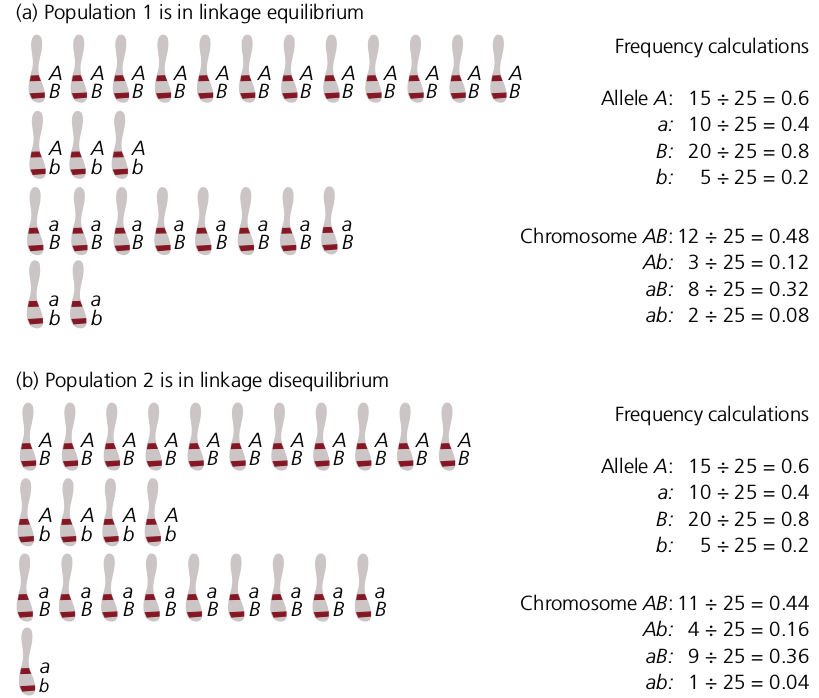
\includegraphics[width=0.82\linewidth]{../images/linkage_disequilibrium_two_pops} \caption{\textbf{Populations with identical allele frequencies, but different chromosome frequencies}. (a) In population 1 the frequency of allele $B$ among $A$-bearing chromosomes (12 of 15, or 0.8) is the same as it is among $a$-bearing chromosomes (8 of 10, or 0.8). (b) In population 2 the frequencies of $B$ among $A$-bearing versus $a$-bearing chromosomes are different (11 of 15, or 0.73, versus 9 of 10, or 0.9). Population 2 is said to be in linkage disequilibrium.}\label{fig:linkage-disequlibrium-example}
\end{figure}

\end{columns}
\end{frame}

\begin{frame}{}
\protect\hypertarget{section-28}{}
\footnotesize

The coefficient of linkage disequilibrium, symbolized by D, is defined
as:

\[
g_{AB}g_{ab} - g_{Ab}g_{aB}
\]

Where \(g_{AB}, g_{ab}, g_{Ab}~\text{and}~g_{aB}\) are the frequencies
of \(AB\), \(ab\), \(Ab\) and \(aB\) chromosomes.

Let \(p\) and \(q\) be frequencies of \(A\) and \(a\), and let \(s\) and
\(t\) be the frequencies of \(B\) and \(b\). If a population is in
linkage equilibrium, then \(g_{AB} = ps\), \(g_{Ab} = pt\),
\(g_{aB} = qs\), and \(g_{ab} = qt\). And furthermore,

\[
D = psqt -ptqs = 0
\] If, the population is in LD, \(D \neq 0\)
(\(0.25 \geq D \geq - 0.25\)). The maximum value occurs when \(AB\) and
\(ab\) are the only chromosomes present and each has a frequency of 0.5.
Minimum value is possible when \(Ab\) and \(aB\) are the only
chromosomes present and each is at a frequency of 0.5.
\end{frame}

\begin{frame}{Equilibrium frequency and linkage disequilibrium}
\protect\hypertarget{equilibrium-frequency-and-linkage-disequilibrium}{}
\begin{columns}[T,onlytextwidth]
\column{0.7\textwidth}

\begin{table}
\centering\begingroup\fontsize{7}{9}\selectfont

\begin{tabular}{>{\raggedleft\arraybackslash}p{2.6em}>{\raggedleft\arraybackslash}p{4.25em}>{\raggedleft\arraybackslash}p{4.25em}>{\raggedleft\arraybackslash}p{3.25em}>{\raggedleft\arraybackslash}p{3.25em}>{\raggedleft\arraybackslash}p{3.25em}>{\raggedleft\arraybackslash}p{3.25em}>{\raggedleft\arraybackslash}p{3.25em}}
\toprule
generation & amount added or subtracted & proportion disequilibrium remaining & gametes AB & gametes Ab & gametes aB & gametes ab & recombination freq\\
\midrule
1 & 0.00 & 1.00 & 0.30 & 0.30 & 0.30 & 0.10 & Inf\\
2 & 0.50 & 0.50 & 0.33 & 0.27 & 0.27 & 0.13 & 0.22\\
3 & 0.75 & 0.25 & 0.34 & 0.26 & 0.26 & 0.15 & 0.08\\
4 & 0.88 & 0.12 & 0.35 & 0.25 & 0.25 & 0.15 & 0.04\\
5 & 0.94 & 0.06 & 0.36 & 0.24 & 0.24 & 0.16 & 0.02\\
\addlinespace
6 & 0.97 & 0.03 & 0.36 & 0.24 & 0.24 & 0.16 & 0.01\\
7 & 0.98 & 0.02 & 0.36 & 0.24 & 0.24 & 0.16 & \\
\bottomrule
\end{tabular}
\endgroup{}
\end{table}

\column{0.3\textwidth}

\begin{figure}

{\centering \includegraphics[width=0.95\linewidth]{07-population_genetics_files/figure-beamer/ld-decay-plot-1} 

}

\caption{With sexual reproduction and random mating, linkage disequilibrium falls over time. The graph shows the level of linkage disequilibrium between two loci over 40 generations in random-mating populations with different rates of recombination, r. The population starts with the coefficient of LD (D) at its maximum possible value, 0.25.}\label{fig:ld-decay-plot}
\end{figure}

\end{columns}
\end{frame}

\begin{frame}{Gametic disequilibrium (or LD)}
\protect\hypertarget{gametic-disequilibrium-or-ld}{}
\begin{itemize}
\tightlist
\item
  Processes that maintain or increase gametic disequilibrium

  \begin{enumerate}
  \tightlist
  \item
    Physical linkage\\
  \item
    Natural selection\\
  \item
    Mutation\\
  \item
    Mixing of diverged populations\\
  \item
    mating system\\
  \item
    Chance
  \end{enumerate}
\end{itemize}

Refer to Varshney, Langridge, and Graner (2007) for a discourse on
population structure using LD, and to Khadka et al. (2020) for that in
relation to spring wheat in Nepal.
\end{frame}

\hypertarget{gentic-load-gentic-death-and-genetic-diversity}{%
\section{Gentic load, gentic death and genetic
diversity}\label{gentic-load-gentic-death-and-genetic-diversity}}

\begin{frame}{Genetic diversity}
\protect\hypertarget{genetic-diversity}{}
(Refer to earlier discussion on Gene Diversity of G6PD locus assessed
using SNP.)
\end{frame}

\begin{frame}{Genetic load}
\protect\hypertarget{genetic-load}{}
\footnotesize

\begin{itemize}
\tightlist
\item
  The difference between the fitness of an average genotype in a
  population and the fitness of some reference genotype, which may be
  either the best present in a population, or may be the theoretically
  optimal genotype.
\item
  The average individual taken from a population with a low genetic load
  will generally, when grown in the same conditions, have more surviving
  offspring than the average individual from a population with a high
  genetic load.
\item
  High genetic load may put a population in danger of extinction.
\item
  Consider \(n\) genotypes \(\mathbf{A}_{1},\dots ,\mathbf{A}_{n}\),
  which have the fitnesses \$ w\_\{1\},\dots ,w\_\{n\}\$ and frequencies
  \(p_{1},\dots, p_{n}\), respectively. Ignoring frequency-dependent
  selection, the genetic load \(L\) may be calculated as:
\end{itemize}

\[
\small
L={{w_{\max }-{\bar {w}}} \over w_{\max }}
\]
\end{frame}

\begin{frame}{}
\protect\hypertarget{section-29}{}
where \(w_{\max }\) is either some theoretical optimum, or the maximum
fitness observed in the population. In calculating the genetic load,
\(w_{1}\dots w_{n}\) must be actually found in at least a single copy in
the population, and \(\bar{w}\) is the average fitness calculated as the
mean of all the fitnesses weighted by their corresponding frequencies:

\[
\small
{\bar {w}}={\sum _{i=1}^{n}{p_{i}w_{i}}}
\]

where the \(i^\mathrm{th}\) genotype is \(\mathbf{A}_{i}\) and has the
fitness and frequency \(w_{i}\) and \(p_{i}\) respectively.
\end{frame}

\begin{frame}{Causes of genetic load}
\protect\hypertarget{causes-of-genetic-load}{}
\begin{itemize}
\tightlist
\item
  Deleterious mutations
\item
  Inbreeding
\item
  Recombination/segregation
\item
  Migration
\end{itemize}
\end{frame}

\begin{frame}{Genetic death}
\protect\hypertarget{genetic-death}{}
\begin{itemize}
\tightlist
\item
  The removal of a gene from the gene pool of a population.
\item
  Can be the result of infertility, failure to reproduce, or death
  before sexual maturity of all indviduals carrying that gene.
\item
  Genetic death is not necessarily associated with poor health or loss
  of life, but rather refers to the impediment of genes being passed on
  to future generations.
\item
  Facilitates natural selection -- loss of harmful genes can be
  beneficial to future generations that are born from that gene pool,
  potentially increasing fitness.
\item
  Examples of genetic death constituting a catalyst for evolution
  include genes can be seen in pathogen resistance, such as the genetic
  loss of certain cellular receptors that inhibit entry of pathogens
  into target cells exhibited in genotypes with malaria or AIDS
  resistance.
\end{itemize}
\end{frame}

\hypertarget{bibliography}{%
\section{Bibliography}\label{bibliography}}

\begin{frame}{References}
\protect\hypertarget{references}{}
\hypertarget{refs}{}
\begin{cslreferences}
\leavevmode\hypertarget{ref-khadka2020population}{}%
Khadka, Kamal, Davoud Torkamaneh, Mina Kaviani, Francois Belzile, Manish
N Raizada, and Alireza Navabi. 2020. ``Population Structure of Nepali
Spring Wheat (Triticum Aestivum L.) Germplasm.'' \emph{BMC Plant
Biology} 20 (1): 1--12.

\leavevmode\hypertarget{ref-varshney2007application}{}%
Varshney, Rajeev K, Peter Langridge, and Andreas Graner. 2007.
``Application of Genomics to Molecular Breeding of Wheat and Barley.''
\emph{Advances in Genetics} 58: 121--55.
\end{cslreferences}
\end{frame}




\end{document}
